\documentclass[a4paper,11pt]{article}

\usepackage[T1]{polski}
\usepackage[utf8]{inputenc}
\usepackage{verbatim}
\usepackage{graphics}
\usepackage{graphicx}
\usepackage{float}
\usepackage[hidelinks]{hyperref}
\usepackage[figurename=Zrzut\ ekranu]{caption}

\hoffset=-3.0cm                         
\textwidth=18cm                         
\evensidemargin=0pt

\voffset=-3cm                           
\textheight=27cm                        

\setlength{\parindent}{0pt}           
\setlength{\parskip}{\medskipamount}    
\raggedbottom              

\title{Raport z projektu indywidaulnego}
\author{Michał Banaszczak}
\date{14 czerwca 2022} 

\begin{document}

\maketitle
\tableofcontents

\section{Cel projektu}
    Pierwotnym celem projektu było przeprowadzenie analizy wyników sportowych
    dotyczących Igrzysk Olimpijskich. Nie mogłem nigdzie jednak znaleźć
    zadowalających zbiorów daych, dlatego cel został poszerzony o utworzenie
    takowego na podstawie informacji z oficjalnych stron IO. W trakcie rozwoju
    projektu jednak spodobały mi się technologie webowe, m.in. Node.js czy
    ekstensywne zastosowanie Chrome DevTools. Z tego względu zdecydowałem się
    ponownie poszerzyć zakres projektu o utworzenie dodatkowego zbioru danych
    na podstawie wyników medalistów z poszczególnych Igrzysk. Wyróżniłem w ten
    sposób 3 kamienie milowe projektu:
    \begin{enumerate}
        \item utworzenie zbioru danych dot. wyników wszystkich nowożytnych IO,
        \item utworzenie zbioru danych medalistów poszczególnych IO,
        \item analiza tych zbiorów
    \end{enumerate}

\section{Struktura stron źródłowych do scrapowania}
\subsection{Strona z wynikami wszystkich Igrzysk}
    W tej aplikacji webowej wszystkie igrzyska, sporty i dyscypliny tworzą
    strukturę drzewa. Przy każdej interakcji guziki są niszczone, a nie chowane.
    Koniecznym jest więc tworzenie po każdej interakcji nowej \verb|HTMLCollection|.
    Podstrony dyscyplin są statyczne.
    \begin{figure}[H]
        \centering
        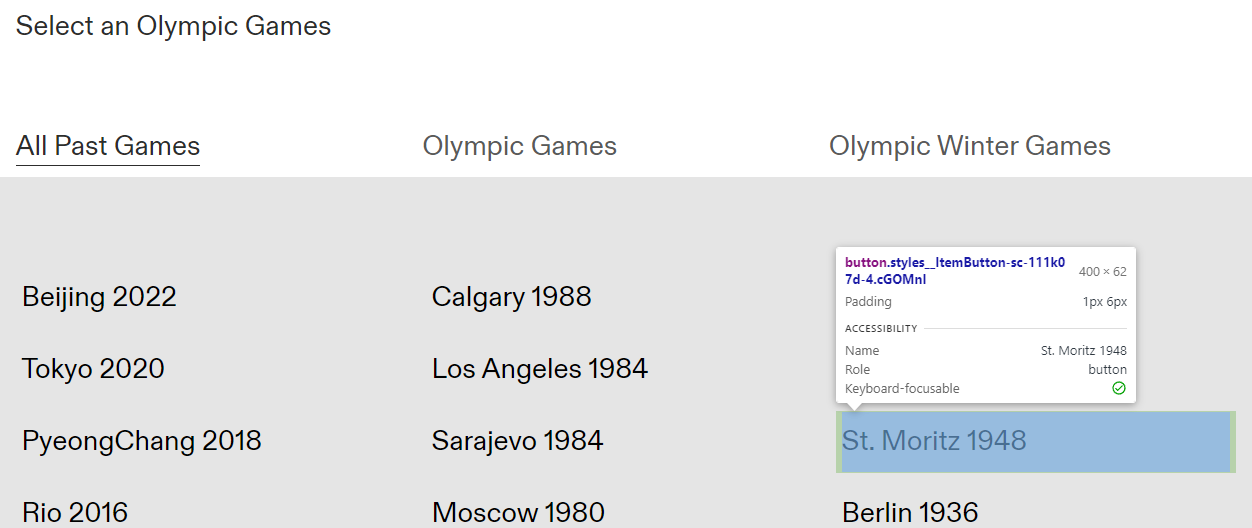
\includegraphics[width=0.8\linewidth]{1-games-list.png}
        \caption{Widok aplikacji przed wybraniem konkretnych igrzysk}
    \end{figure}

    \begin{figure}[H]
        \centering
        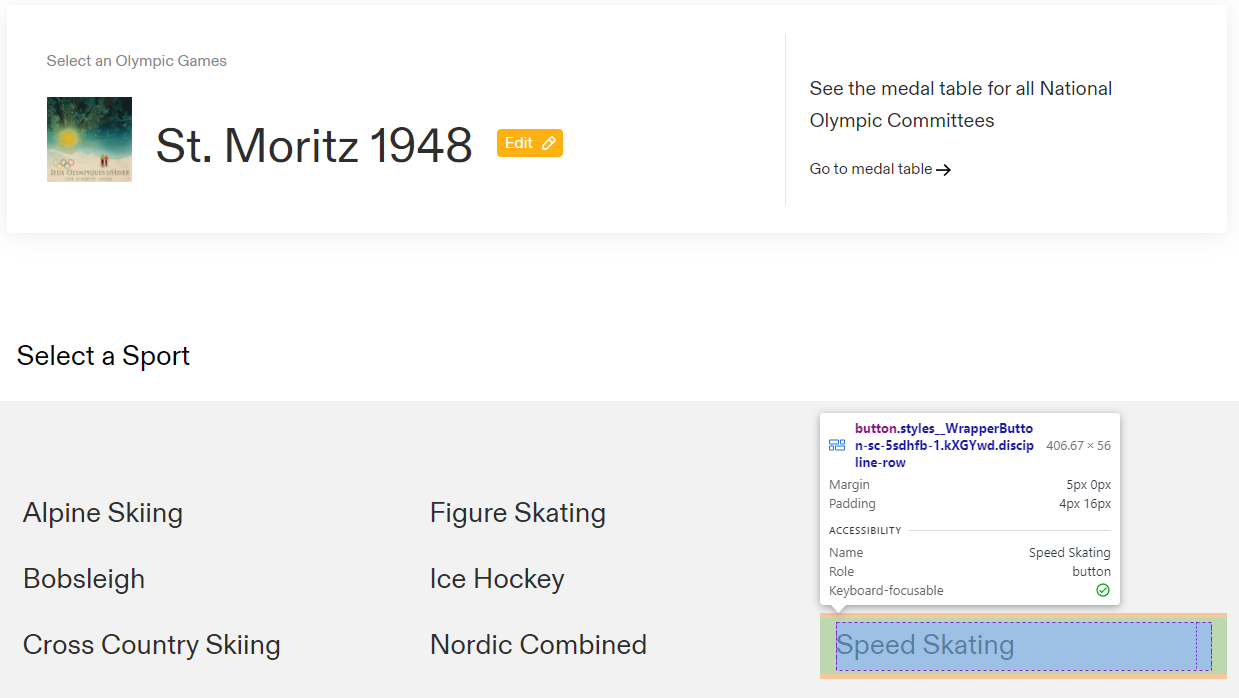
\includegraphics[width=0.8\linewidth]{1-sport-list.png}
        \caption{Lista sportów po wybraniu konkretnych igrzysk}
    \end{figure}

    \begin{figure}[H]
        \centering
        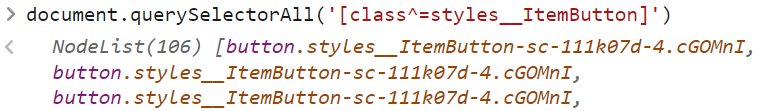
\includegraphics[width=0.5\linewidth]{1-selector-on-games-list.png}
        \caption{Lista elemntów poszczególnych IO przed interakcją}
    \end{figure}

    \begin{figure}[H]
        \centering
        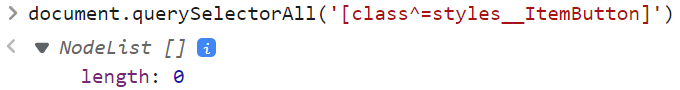
\includegraphics[width=0.5\linewidth]{1-selector-on-sports-list.png}
        \caption{Lista elemntów poszczególnych IO po interakcji}
    \end{figure}

\subsection{Strona z wynikami medalistów}
    Na stronie z wynikami medalistów znajduje się aplikacja z listą zawodników,
    która przy każdym doładowaniu powiększa się o kolejnych dziesięciu atletów.
    Guzik do ładowania dalszej części listy (oczywiście) jest niszczony i później
    tworzony nowy. Aplikacja ma buga, który powoduje ponowne załadowanie ostatnio
    pobranych atletów przy zmianie karty, jednak nie wpłynie on na działanie
    scrapera. Podstrony z danymi sportowców są statyczne, natomiast ilość wierszy
    tabeli z danymi nie zawsze jest równa i nie mają one charakterystycznych
    klas, więc trzeba przeiterować przez wszystkie w poszukiwaniu interesujących 
    nas danych.
    \begin{figure}[H]
        \centering
        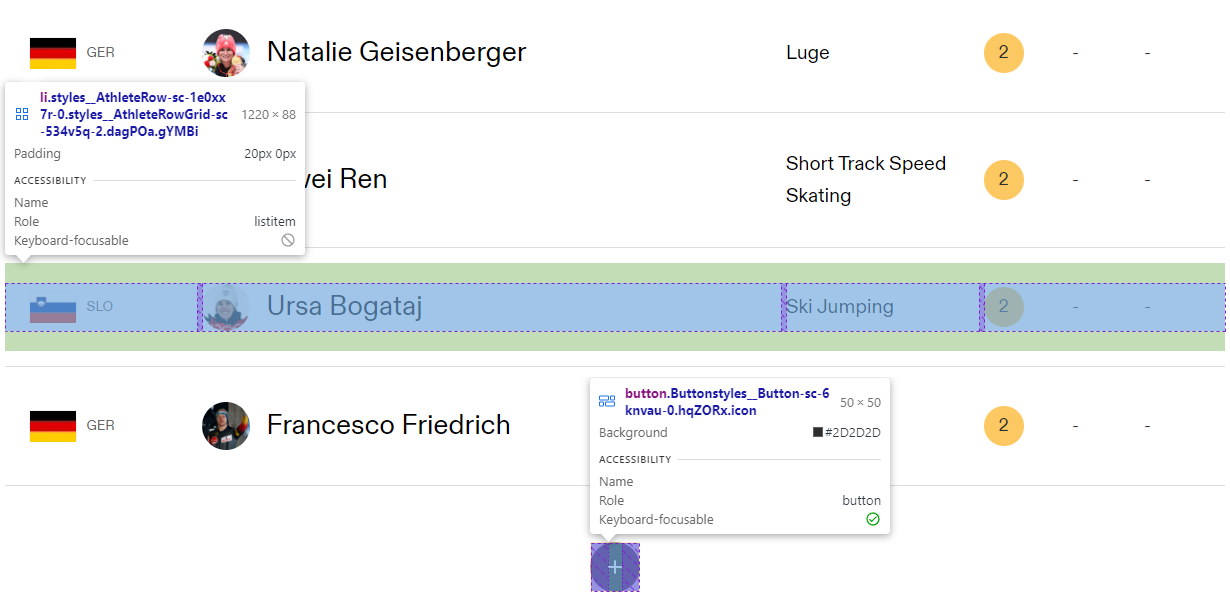
\includegraphics[width=0.8\linewidth]{2-fragmentlisty.png}
        \caption{Fragment listy zawodników}
    \end{figure}

    \begin{figure}[H]
        \centering
        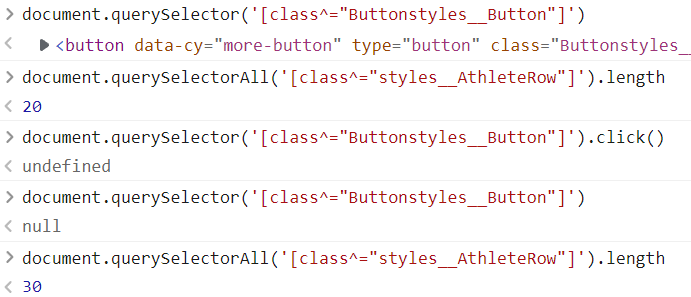
\includegraphics[width=0.5\linewidth]{2-zachowanielisty.png}
        \caption{Zachowanie strony przy doładowywaniu kolejnych zawodników}
    \end{figure}

\section{Działanie scraperów}
\subsection{Wykorzystane technologie}
Wszystkie scrapery oparte są na tych samych technologiach - środowisku Node.js
v17.9.0 oraz bibliotece Puppeteer v13.5.2. Ten z kolei korzysta z silnika
przeglądarkowego Chromium 100.0.4889.0.

\subsection{Proces scrapowania wszystkich wyników}
    Ze względu na specyfikę aplikacji webowej z wynikami Igrzysk Olimpijskich i 
    rozmieszczenie danych na tysiącach podstron, scrapowanie zostało podzielone
    na dwa etapy.
    \begin{enumerate}
        \item Zadaniem skryptu \verb|linkRetriever.js| było przejście przez
        \textit{drzewo} aplikacji głównej strony z wynikami wykorzystując algorytm
        DFS, zbierając macierz danych z wyszczególnionymi kolumnami
        \verb|[Host, Rok,|\newline\verb|Typ, Sport, Dyscyplina, Link]|. Przez
        konieczność wykonania całego skrapowania wewnątrz skryptu ewaluacyjnego,
        przerwanie działania skryptu przed ukończeniem skutkuje utratą wszystkich
        danych. Skutkiem działania jest plik \verb|eventlinks.csv| z 6575
        wierszami danych.
        \item Skrypt \verb|scoreRetriever.js| iteruje przez linki zebrane przez 
        poprzedni skrypt i rozrzesza zbiór danych o kolumny
        \verb|[Miejsce, Państwo, Sportowiec, Wynik, Przypisy]|. Poszczególne
        strony  zawierają jedynie zawartość statyczną, dzięki czemu zebrane dane
        można zapisywać w trakcie scrapowania, a w razie błędów po drodze nie
        traci się dotychczasowych postępów scrapowania. Pomocna funkcjonalność
        biorąc pod uwagę, że plik wynikowy, \verb|scoresFromAllGamesNotParsed.csv|,
        ma ostatecznie 162473 wierszy. Skrypt ten nie zajmuje się formatem danych. 
    \end{enumerate}
\subsection{Formatowanie wyników}
    Formatem plików zajmuje się moduł \verb|scoreFormatter.js|. Dla łatwiejszej
    analizy danych zastosowano poniższe przekształcenia:
    \begin{itemize}
        \item zamiana kodów państw na pełne nazwy
        \item zamiana nazw medali na numer miejsca
        \item usunięcie \textit{=} z numerów miejsc zajętych ex aequo
        \item kapitalizacja pierwszych lilter nazwisk sportowców
        \item wyniki w formacie \textit{min:sek.setnesek} na \textit{sek.setnesek}
        \item jeśli istniał przypis tłumaczący brak wyniku, to zostawał wpisany
              w miejsce takowego
    \end{itemize}
    Oczywiście setki różnych dyscyplin miały setki różnych sposobów na zapis
    wyniku i setki sposobów na ich interpretację. Analiza i przekształcanie 
    wszystkich rodzajów wyników wykroczyłaby poza ramy czasowe tego projektu.
    Wykonano tylko format jednego z częściej używanych zapisów jako \textit{proof
    of concept}.
\subsection{Proces scrapowania zawodników}
    Tak samo jak dla wyników wszystkich dyscyplin, strona z medalistami
    poszczególnych IO wykorzystuje mechanizm dynamiczengo doładowywania zawartości
    w trakcie przeglądania. Analogicznie więc scrapowanie zostało podzielone na
    dwa etapy, jednak przez mniejszą objętość danych zajmuje się nimi jeden skrypt
    - \verb|athleteRetriever.js|. Jest on zdolny do scrapowania danych ze
    wszystkich nowożytnych IO, ale trzeba podmienić link do właściwej strony.
    \begin{enumerate}
        \item Pierwszy etap polega na rozwinięciu całej tabeli wyników, która 
        przy każdym wciśnięciu guzika powiększa się o 10 wierszy. Cała tabela
        zostaje zwrócona ze skryptu ewaluacyjnego w postaci macierzy o kolumnach
        \verb|[Kraj, Sportowiec, Sport, Złoto, Srebro, Brąz, Link]|.
        \item Teraz iterując po wierszach macierzy przechodzimy po podstronach
        każdego ze sportowców, zbierając stamtąd kolejne dane. Macierz zostaje
        powiększona o kolumny \verb|[Wzięto udział, Rok urodzenia]| i zapisano
        do pliku \verb|medalistsYEARNotParsed.csv|.
    \end{enumerate}
    Format plików jest dostosowany do kolumn nowej tabeli natomiast proces 
    przebiega tak samo, jak wyżej, więc nie będę go ponownie opisywał. Sformatowany
    plik zostaje zapisany jako \verb|medalistsYEAR.csv|.
\subsection{Trudności i ograniczenia}
    Podstawowym problemem jaki stanowiła oficjalna strona z wynikami Igrzysk
    Olimpijskich jest ilość dynamicznego contentu i mutacji strony jakie zachodzą
    przy każdym kliknięciu. Ten problem rozwiązano przez zastosowanie
    MutationObservera, który nasłuchiwał zmian na stronie - w pierwszym scraperze
    jakichkolwiek, a w drugim konkretnie pojawienia się guzika do dalszego
    ładowania tabeli.
    \newline
    Kolejnym ograniczeniem była funkcjonalność metody \verb|Page.evaluate()|,
    czy raczej właśnie brak funkcjonalności. Funkcja zwrotna podawana jako 
    pierwszy argument metody jest wstrzykiwana do strony jako skrypt ewaluacyjny.
    Jeśli ta funkcja przyjmuje parametry pochodzące z Node'owego środowiska, to 
    należy je podać jako kolejne argumenty metody - również zostaną wstrzyknięte
    do przeglądarki i skrypt ewaluacyjny będzie miał do nich dostęp. Nie dotyczy
    to niestety referencji do funkcji - te nie zostają przeniesione. Z tego 
    względu funkcje wykorzystywane w skrypcie ewaluacyjnym musiały zostać 
    zdefiniowane wewnątrz callbacka, tworząc tzw. \textit{pyramid of doom}.
    \newline
    Oczywistym jest również konieczność korzystania w takim zastosowaniu z
    asynchroniczności JavaScriptu. Wykorzystywałem do tego głównie Promise'y oraz 
    składnię async/await wprowadzone kolejno w ECMAScript 6 i 2017 (w międzyczasie
    zmieniono sposób nazywania nowych wydań). Mimo tego nie udało mi się uciec
    od tzw. \textit{callback hell} - w rekordowym miejscu występuje 6 zagnieżdżeń
    funkcji zwrotnych. Trzeba jednak przyznać, że zdecydowanie jest to nietypowe
    zastosowanie składni JSa.
    
\section{Analiza zbioru}
    Technologie wykorzystywane do analizy to Jupyter Notebook z iPythonem 3.10.0.
    W głównej mierze wykorzystywano biblioteki NumPy, Pandas, Matplotlib.
    Przeprowadzono analizę i wizualizację na danych z utworzonego zbioru, ale 
    w niektórych punktach odnoszono się także do dodatkowych źródeł (wszystkie
    załączone w bibliografii). Po dokładny opis analizowanych zagadnień odsyłam 
    do pliku \verb|allGamesAnalysis.ipynb| lub \verb|analizaWynikowIO.html|.
    Wykorzystywane środowisko pozwala na integrację kodu z opisami i wizualizacją,
    w związku z czym nie chcę bez sensu powtarzać tu treści.

\section{Refleksje}
    Dane zawarte na oficjalnych stronach IO wbrew oczekiwaniom są bardzo
    niespójne, konwencje nazewnicze sportów i dyscyplin różnią się w latach,
    tak samo formaty zapisu wyników. Tych w starszych Igrzyskach często zwyczajnie
    brakuje. W różnych miejscach aplikacji podawane są pełne nazwy państw biorących
    udział, a w innych skrótowce, w dodatku niezgodne ze standardem ISO 3166. 
    Wszystko to znacząco utrudniało przygotowanie zbioru danych, jak również jego
    analizę. \hfill \break
    Dzięki temu uważam, że projekt dał mi solidne zrozumienie podstaw 
    akwizycji danych i problemów jakie można napotkać przy web-scrapingu - zwłaszcza,
    że większość udało mi się rozwiązać i ujednolicić zbiory danych. 
    Z projektu wynoszę dobre zrozumienie działania asynchroniczności w JavaScripcie,
    a także funkcjonalności biblioteki Puppeteer. \hfill \break
    Do analizy danych odnoszę wrażenie równie dobrze nadałby się tu SQL - tak
    naprawdę to w większości przypadków naśladowałem atrybutem \verb|pd.DataFrame.loc|
    zachowanie \verb|WHERE|. Jupyter Notebook ma jednak tą przewagę, że analiza, 
    wizualizacja i opis słowny danych może znajdować się w tym samym dokumencie,
    co znacznie ułatwia tworzenie takich analiz i późniejsze ich czytanie. \hfill \break
    Nie zdążyłem jednak wszystkich swoich pomysłów z analizy danych wdrożyć w
    życie. Przykładowe zależności, na których zbadanie brakło mi czasu:
    \begin{itemize}
        \item histogramy czasów dla jakiejś wybranej dyscypliny, zmiana wyników
        wraz z upływem lat
        \item ilość medalistów w zależności od kontynentu
        \item wpływ dopingu na wyniki rosyjskich sportowców na przestrzeni lat
        (zrobiłem tylko dla stałego punktu w czasie)
        \item zależność między wiekiem sportowców, a ilością zdobytych medali
    \end{itemize}
    Wierzę jednak, że gdybym przeanalizował te punkty, wymyśliłbym kolejne i tak
    mógłbym w kółko, a analiza, którą przeprowadziłem rozpatruje ciekawe aspekty
    zebranych danych. Konkludując, uważam że cele projektu zostały spełnione w 
    zadowalającym stopniu, a ja sam wynoszę z niego znajomość nowych technologii.

\newpage
\section{Bibliografia i źródła wykorzystywane w projekcie}
\begin{enumerate}
    \item \href{https://olympics.com/en/olympic-games/olympic-results}{Oficjalna strona IO z wynikami}
    \item \href{https://olympics.com/en/olympic-games/beijing-2022/athletes}{Oficjalna strona IO z medalistami}
    \item \href{https://pptr.dev/}{Dokumentacja Puppeteera}
    \item \href{https://pandas.pydata.org/docs/reference/index.html}{Dokumentacja Pandas}
    \item \href{https://matplotlib.org/stable/api/pyplot_summary.html}{Dokumentacja Pyplot}
    \item \href{https://en.wikipedia.org/wiki/Demographics_of_the_Soviet_Union#Ethnic_groups}{Populacja państw członkowskich ZSRR, stan na 1989}
    \item \href{https://en.wikipedia.org/wiki/Dissolution_of_the_Soviet_Union#Chronology_of_declarations}{Państwa członkowskie ZSRR i daty wystąpień}
\end{enumerate}

\end{document}